\documentclass[a4paper,12pt]{article}

\usepackage{fontspec}
\usepackage{polyglossia}
\setmainlanguage{russian}
\setotherlanguage{english}

% Set main font (Latin)
\setmainfont{Times New Roman} % or any other Latin font you like

% Set font for Cyrillic script explicitly
\newfontfamily\cyrillicfont{Times New Roman} % this font supports Cyrillic on most systems
\newfontfamily\cyrillicfonttt{Courier New} % Or another monospace font that supports Cyrillic


\usepackage{amsmath, amssymb, amsfonts, graphicx, csquotes, array, geometry, titlesec, biblatex, listings, hyperref, caption, xcolor, import, subcaption}

\addbibresource{references.bib} % Файл со списком литературы

\geometry{left=25mm,right=20mm,top=25mm,bottom=25mm}

\begin{document}

\setcounter{page}{2}

\section*{Информация о составе проектной команды, контакты}
\textbf{Руководитель проекта:} Писарев Василий Вячеславович, ведущий научный сотрудник, Международная лаборатория САММА, НИУ ВШЭ

\textbf{Контакт:} vpisarev@hse.ru

\smallskip

\textbf{Студент-исследователь:} Панов Михаил Федорович, студент 2 курса магистратуры по направлению "Системный анализ и математические технологии", МИЭМ НИУ ВШЭ

\textbf{Контакт:} mfpanov@edu.hse.ru

\section*{Реферат}
\subsection*{Объект и предмет исследования:}
Объектом исследования являются бинарные и многокомпонентные смеси, содержащие углекислый газ и н-алканы. Предмет исследования — параметры парного взаимодействия (коэффициенты $k_{ij}$) в уравнении состояния CP-PC-SAFT.

\subsection*{Цель проекта:}
Разработка и проверка методики подбора коэффициентов парного взаимодействия углеводородов с углекислым газом для повышения точности модели CP-PC-SAFT при расчетах фазовых равновесий.

\subsection*{Задачи проекта:}
\begin{itemize}
\item Сбор экспериментальных данных по фазовым диаграммам из базы ThermoML.
\item Обработка данных с использованием библиотеки ThermoPyL.
\item Расчет параметров чистых веществ для CP-PC-SAFT.
\item Оптимизация коэффициентов $k_{ij}$.
\item Сравнение результатов с моделью Брусиловского.
\item Поиск корреляций между $k_{ij}$ и физико-химическими свойствами компонентов.
\item Проверка работоспособности модели на трехкомпонентных смесях.
\end{itemize}

\subsection*{Используемые методы:}
\begin{itemize}
\item Термодинамическое моделирование на основе CP-PC-SAFT и CubicEoS библиотек для Julia.
\item Численная оптимизация и обработка экспериментальных данных с использованием Python и библиотеки ThermoPyL.
\end{itemize}

\subsection*{Результаты проекта:}
\begin{itemize}
\item Подобраны оптимальные коэффициенты $k_{ij}$ для $\mathrm{CO}_{2}$–алканов (от гексана до додекана).
\item Разработан и протестирован код для обработки и анализа данных.
\item Модель CP-PC-SAFT с подобранными $k{ij}$ продемонстрировала точность, сопоставимую или превосходящую уравнение Брусиловского.
\end{itemize}

\subsection*{Новизна и практическая значимость:}
\begin{itemize}
\item Модель CP-PC-SAFT использована с расчетными параметрами веществ без подбора, что упрощает параметризацию.
\item Автоматизированный pipeline для обработки ThermoML-данных.
\end{itemize}

\textbf{Области применения:} Химическая инженерия, нефтехимия, моделирование энергетических процессов.

\textbf{Степень готовности:} Метод протестирован, код написан, база данных создана. Готов к использованию в научных исследованиях и для адаптации в инженерных расчетах.

\tableofcontents
\newpage
\section{Введение}

\subsection{Аналитический обзор научно-технической информации}

\subsection{Используемые базы данных и инструменты обработки данных}

\subsubsection{База данных ThermoML}

ThermoML — это стандартизированный формат представления термодинамических данных, разработанный и поддерживаемый Национальным институтом стандартов и технологий США (NIST) \cite{Frenkel2004}. Он предоставляет машиночитаемый способ хранения экспериментальных данных о фазовых равновесиях, плотностях, давлениях, мольных долях, температурах и других свойствах веществ и смесей \cite{Chirico2020}. В контексте данного проекта база ThermoML используется как основной источник экспериментальных фазовых диаграмм бинарных систем $\mathrm{CO}_2$–алкан. Стандартизованный формат позволяет извлекать данные программно, без ручной предобработки.

\subsubsection{Библиотека ThermoPyL}

ThermoPyL — это свободно распространяемая Python-библиотека, разработанная для автоматического парсинга и обработки данных ThermoML \cite{Picard2015}. Она предоставляет удобные функции для извлечения, фильтрации, группировки и конвертации термодинамических данных из XML-файлов в удобные форматы (например, pandas DataFrame), а также предоставляет доступ к информации о фазах, составах, давлениях и других параметрах.

В рамках проекта ThermoPyL использовалась для:
\begin{itemize}
\item автоматического чтения XML-файлов ThermoML;
\item фильтрации данных по фазе и составу;
\item группировки данных по экспериментам;
\item подготовки входных данных для модели CP-PC-SAFT.
\end{itemize}

Использование библиотеки позволило исключить ручную предобработку, сократить количество ошибок и автоматизировать подготовку данных для моделирования.

\subsection{Описание модели CP-PC-SAFT}

Уравнение состояния PC-SAFT используется для моделирования фазовых равновесий многокомпонентных смесей. В классическом подходе параметры веществ подбираются по экспериментальным данным, однако метод CP-PC-SAFT позволяет вычислять их на основе критической точки и температуры кипения, что избавляет от необходимости ручной подгонки.

Для корректного моделирования фазового равновесия в смесях требуются коэффициенты парных взаимодействий \( k_{ij} \), которые влияют на предсказание растворимости компонентов. В рамках проекта была проведена оптимизация значений \( k_{ij} \) для систем $\mathrm{CO}_{2}$ с алканами, что позволило повысить точность расчётов.

\subsubsection{Основные положения}

CP-PC-SAFT (Critical Point Perturbation Chain SAFT) — это модифицированная версия уравнения состояния PC-SAFT, предназначенная для точного расчёта параметров чистого вещества на основе данных о его критической точке и температуре кипения. В отличие от классического PC-SAFT, где параметры веществ подбираются эмпирически по экспериментальным данным, CP-PC-SAFT позволяет вычислять их, снижая зависимость от ручной подгонки.

\subsubsection{Уравнение состояния PC-SAFT}

Основное уравнение состояния PC-SAFT выражается через вклад свободной энергии Гельмгольца \( a \):

\begin{equation}
a(v, T) = a^{\text{id}} + a^{\text{hs}} + a^{\text{chain}} + a^{\text{disp}} + a^{\text{assoc}}
\end{equation}

Где:
\begin{itemize}
    \item \( a^{\text{id}} \) — вклад идеального газа;
    \item \( a^{\text{hs}} \) — вклад жёстких сфер;
    \item \( a^{\text{chain}} \) — вклад цепных взаимодействий;
    \item \( a^{\text{disp}} \) — вклад дисперсионных сил;
    \item \( a^{\text{assoc}} \) — вклад ассоциативных взаимодействий (учитывает водородные связи).
\end{itemize}

\subsubsection{Параметры веществ}

В рамках CP-PC-SAFT каждое вещество описывается тремя основными параметрами:
\begin{itemize}
    \item \( m \) — число сегментов в молекуле;
    \item \( \sigma \) — эффективный диаметр сегмента молекулы;
    \item \( \varepsilon \) — энергия взаимодействия между сегментами.
\end{itemize}

Эти параметры определяются через критическую точку и температуру кипения вещества, а не через эмпирическую подгонку, что делает модель более универсальной.

\subsubsection{Критерии параметризации в CP-PC-SAFT}

В модели CP-PC-SAFT параметры вещества корректируются так, чтобы соответствовать следующим условиям \cite{polishuk2014standardized}:

\begin{equation}
\left( \frac{\partial P}{\partial v} \right)_{T_c} = 0, \quad
\left( \frac{\partial^2 P}{\partial v^2} \right)_{T_c} = 0
\end{equation}

\begin{equation}
P_c = P_{\text{c, exp}}
\end{equation}

\begin{equation}
\rho_{\text{liq, triple}} = \rho_{\text{liq, triple, exp}}
\end{equation}

Здесь:
\begin{itemize}
    \item \( P_c \) — давление в критической точке;
    \item \( T_c \) — критическая температура;
    \item \( \rho_{\text{liq, triple}} \) — жидкостная плотность в тройной точке.
\end{itemize}

\subsubsection{Парное взаимодействие между компонентами смеси}

При описании смесей используется коэффициент парного взаимодействия \( k_{ij} \), который учитывает отклонение от идеального поведения и корректирует дисперсионный параметр:

\begin{equation}
	(\varepsilon/k)_{ij} = (1 - k_{ij}) \sqrt{(\varepsilon/k)_i (\varepsilon/k)_j}
\end{equation}

Оптимизация коэффициента \( k_{ij} \) является ключевой задачей данной работы, поскольку он напрямую влияет на точность предсказания фазового равновесия в смесях алкан–$\mathrm{CO}_2$.

\subsubsection{Применимость модели CP-PC-SAFT}

CP-PC-SAFT широко применяется для моделирования фазовых равновесий в системах углеводородов, $\mathrm{CO}_{2}$ и других полярных компонентов. Данный подход позволяет:
\begin{itemize}
    \item Уменьшить зависимость модели от эмпирической подгонки;
    \item Улучшить предсказание фазовых диаграмм за счёт учёта критической точки;
    \item Использовать универсальные параметры, применимые к широкому классу веществ.
\end{itemize}

\subsubsection{Особенности и область применения}

Модель SAFT применяется в:
\begin{itemize}
    \item расчётах фазовых диаграмм (VLE, LLE, SLE);
    \item прогнозировании растворимости газов и жидкостей;
    \item описании поведения полимеров, водородно-связанных систем и смесей высокой сложности.
\end{itemize}

Преимущества:
\begin{itemize}
    \item физическая интерпретация параметров;
    \item высокая точность при наличии ассоциации или сложной структуры компонентов;
    \item применимость к широкому классу веществ.
\end{itemize}

Недостатки:
\begin{itemize}
    \item необходимость подбора большого количества параметров;
    \item более высокая вычислительная стоимость по сравнению с кубическими моделями.
\end{itemize}

\textbf{Источники данных:} \\
\begin{itemize}
	\item Модель SAFT и её модификации реализованы с использованием библиотеки \texttt{cp\_pc\_saft} (Julia). Теоретическая база изложена в фундаментальных публикациях и документации к используемому коду. \cite{cp_pc_saft2024}
    \item Gross J., Sadowski G. (2001) – Уравнение состояния PC-SAFT Эта работа представляет собой фундаментальное исследование, в котором предлагается уравнение состояния PC-SAFT (Perturbed-Chain SAFT). Авторы применили теорию возмущения для моделирования поведения цепных молекул, что позволило существенно повысить точность термодинамических расчетов, особенно для сложных смесей. \cite{Gross2001}
     \item Held C. et al. (2014) – Модифицированное уравнение PC-SAFT Авторы предлагают модифицированную версию уравнения состояния PC-SAFT, основанную на данных о критической точке. Это исследование направлено на улучшение предсказательных способностей модели, особенно для сложных многокомпонентных систем. Данная работа играет ключевую роль в моделировании фазового равновесия для углеводородных смесей. \cite{Held2014}
\end{itemize}

\subsection{Описание уравнения состояния Брусиловского}

\subsubsection{Основные положения}

Уравнение состояния Брусиловского представляет собой модифицированное кубическое уравнение состояния, применяемое для описания фазовых равновесий в многокомпонентных смесях. Оно является одной из версий уравнений Ван-дер-Ваальсовского типа, адаптированных для инженерных задач, особенно в нефтехимии и переработке углеводородов.

Главная особенность модели заключается в её эмпирической точности при относительно низкой вычислительной стоимости. В отличие от моделей типа SAFT, уравнение Брусиловского не включает явного микроскопического описания структуры молекул, но хорошо справляется с задачами расчета равновесия жидкость–пар в практических условиях.

\subsubsection{Уравнение состояния}

Уравнение Брусиловского использует следующую формулу для давления:

\begin{equation}
P = \frac{RT}{v - b} - \frac{a(T)}{v(v + b)}
\end{equation}

где:
\begin{itemize}
    \item \( P \) — давление,
    \item \( T \) — температура,
    \item \( v \) — молярный объем,
    \item \( R \) — универсальная газовая постоянная,
    \item \( a(T) \), \( b \) — параметры вещества, зависящие от критических свойств.
\end{itemize}

Функция \( a(T) \) обычно задаётся через температурную зависимость с использованием редуцированных температур и дополнительных эмпирических коэффициентов. Параметры \( a \) и \( b \) рассчитываются на основе критической температуры, давления и температуры кипения вещества.

\subsubsection{Особенности и область применения}

Модель применяется для:
\begin{itemize}
    \item расчета фазовых равновесий (VLE — vapor-liquid equilibrium);
    \item оценки растворимости газов в жидкостях;
    \item моделирования термодинамических свойств смесей углеводородов.
\end{itemize}

Преимущества:
\begin{itemize}
    \item простота реализации и высокая скорость расчета;
    \item хорошая согласованность с экспериментальными данными для систем на основе алканов;
    \item устойчивая работа при умеренных давлениях и температурах.
\end{itemize}

Недостатки:
\begin{itemize}
    \item отсутствие физической интерпретации параметров;
    \item снижение точности для сложных полярных соединений и водородно-связанных систем;
    \item необходимость подбора бинарных коэффициентов для смесей.
\end{itemize}

\textbf{Источники данных:} \\
Модель реализована и протестирована с использованием библиотеки \texttt{CubicEoS} (Python). Теоретическая база приведена в учебной и справочной литературе по термодинамике углеводородов, например:

\begin{itemize}
    \item Брусиловский Г. Я., \"Термодинамика углеводородов и их смесей\", М.: Недра, 1987. \cite{Brusilovskii1987}
    \item Документация к библиотеке \texttt{CubicEoS}. \cite{Pisarev2025} \cite{Zakharov2024}
\end{itemize}


\subsection{Актуальность и новизна}

Оптимизация коэффициентов парного взаимодействия \( k_{ij} \) необходима для повышения точности фазового моделирования, особенно для систем углеводородов с $\mathrm{CO}_{2}$, которые широко используются в нефтехимической и газовой промышленности.

В рамках работы были проведены:
\begin{itemize}
	\item сбор и предварительная обработка экспериментальных данных по фазовым диаграммам из базы ThermoML;
	\item расчет параметров веществ для CP-PC-SAFT;
	\item численная оптимизация коэффициента \( k_{ij} \) для улучшения точности прогнозирования фазовых равновесий.
\end{itemize}

Результаты показали, что использование оптимизированного коэффициента \( k_{ij} \) в CP-PC-SAFT улучшает предсказание давления насыщения и фазового состава, а также позволяет конкурировать с промышленными моделями, такими как уравнение состояния Брусиловского.

\section{Основная часть}

\subsection{Описание решения задач разработки/исследований}

В рамках проекта была проведена параметризация коэффициентов парного взаимодействия \( k_{ij} \) для модели CP-PC-SAFT с целью повышения точности предсказания фазовых равновесий в смесях алкан–$\mathrm{CO}_{2}$.

Работа включала несколько этапов:
\begin{itemize}
    \item Сбор и обработка экспериментальных данных:
    \begin{itemize}
        \item Были получены фазовые диаграммы углеводородов с $\mathrm{CO}_{2}$ из базы данных ThermoML.
        \item Данные прошли предварительную фильтрацию и обработку с использованием библиотеки ThermoPyL.
    \end{itemize}
    \item Расчет параметров веществ:
    \begin{itemize}
        \item Для каждого компонента смеси были определены параметры модели SAFT (число сегментов \( m \), эффективный диаметр \( \sigma \) и энергия взаимодействия \( \varepsilon \)).
	\item
		\begin{table}[ht]
		    \centering
		    \caption{Параметры веществ в CP-PC-SAFT}
		    \begin{tabular}{|l|c|c|c|c|c|c|}
		        \hline
		        \textbf{Вещество} & \textbf{$m$} & \textbf{$\varepsilon/k$} & \textbf{$\sigma$} & \textbf{$\delta$} & \textbf{$T_{\text{тр}}$ (K)} & \textbf{Молекулярная масса} \\
		        \hline
		        Гексан  & 3.511  & 218.238 & 3.656 & 1.161 & 178.0  & 86.18 \\
		        Гептан  & 4.070  & 220.494 & 3.635 & 1.166 & 182.6  & 100.21 \\
		        Октан   & 4.455  & 225.287 & 3.679 & 1.179 & 216.4  & 114.23 \\
		        Нонан   & 4.851  & 229.271 & 3.705 & 1.187 & 219.9  & 128.26 \\
		        Декан   & 5.270  & 232.262 & 3.722 & 1.203 & 243.5  & 142.28 \\
		        Додекан & 6.012  & 238.240 & 3.770 & 1.225 & 263.6  & 170.34 \\
		        \hline
		    \end{tabular}
		\end{table}

    \end{itemize}
    \item Оптимизация коэффициента \( k_{ij} \):
    \begin{itemize}
        \item Выполнена численная оптимизация коэффициента парного взаимодействия, обеспечивающая минимальное отклонение расчетных данных от экспериментальных.
    \end{itemize}
    \item Сравнение с альтернативной моделью:
    \begin{itemize}
        \item Проведено сопоставление точности CP-PC-SAFT с кубическими уравнениями состояния, в частности, с моделью Брусиловского.
    \end{itemize}
    \item Оценка точности на тройных системах:
    \begin{itemize}
	\item Данные для тройных систем не удалось найти в скачанных частях архива ThermoML, поэтому они были вручную собраны из работ \cite{SanchezGarcia2023, Nagarajan1990}. 
        \item Проведен анализ точности предсказания мольных долей в тройной системе $\mathrm{CO}_{2}$-бутан-декан.
        \item Выполнено сравнение точности вычисления точки кипения в тройных системах $\mathrm{CO}_{2}$-гексан-декан и $\mathrm{CO}_{2}$-октан-декан.
    \end{itemize}

\end{itemize}

\subsection{Описание полученных результатов}

Результаты исследования показали:
\begin{itemize}
    \item Оптимальные значения коэффициента \( k_{ij} \):
    \begin{itemize}

\item Для нахождения оптимального значения коэффициента парного взаимодействия \( k_{ij} \) была реализована процедура оценки точности модели CP-PC-SAFT на экспериментальных данных.

Для каждого фиксированного значения \( k_{ij} \) рассчитывались мольные доли $ \mathrm{CO}_2 $ в жидкой и газовой фазе при различных температурах. Затем вычислялось среднеквадратичное отклонение (MSE) между расчетными и экспериментальными мольными долями по формуле:

\[
\mathrm{MSE}(k_{ij}, T) = \frac{1}{n} \sum_{i=1}^{n} \left(x_{i}^{\text{exp}}(T) - x_{i}^{\text{calc}}(T, k_{ij})\right)^2
\]

где:
\begin{itemize}
    \item $x_{i}^{\text{exp}}(T)$ — экспериментальная мольная доля $ \mathrm{CO}_2 $ при температуре $T$ и $i$-ом давлении,
    \item $x_{i}^{\text{calc}}(T, k_{ij})$ — расчетная мольная доля по модели CP-PC-SAFT с параметром $k_{ij}$ при той же температуре и давлении,
    \item $n$ — число экспериментальных точек по давлению при данной температуре.
\end{itemize}

Для получения единственной метрики ошибки на каждом \( k_{ij} \), eассчитывались MSE в жидкой и газовой фазе отдельно, их сумма усреднялась по всем доступным температурам:

\[
\mathrm{Score}(k_{ij}) = \frac{1}{T} \sum_{t\in T}^{} \left( \mathrm{MSE}_\text{liq}^{(j)}(k_{ij}, t) + \mathrm{MSE}_\text{vap}^{(j)}(k_{ij}, t) \right)
\]

Зависимость $\mathrm{Score}(k_{ij})$ аппроксимировалась с помощью полинома третьей степени, чтобы определить минимум — оптимальное значение коэффициента \( k_{ij} \).

\vspace{1em}
\begin{figure}[ht]
    \centering
    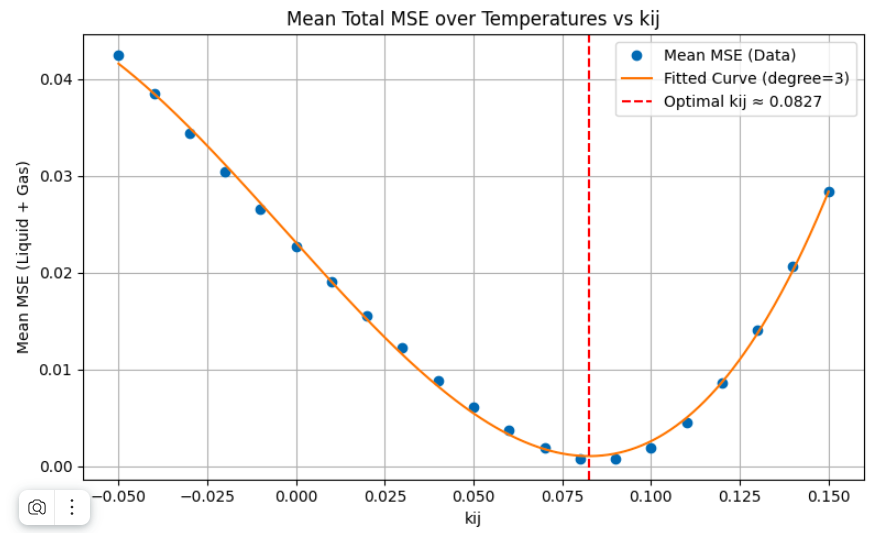
\includegraphics[width=0.6\textwidth]{images/best_kij_heptane.png}
    \caption{Пример нахождения оптимального значения $k_{ij}$ по минимуму средней ошибки для смеси гептан-$ \mathrm{CO}_2 $}
    \label{fig:kij_optimization}
\end{figure}
\vspace{1em}

Ниже представлены оптимальные значения \( k_{ij} \), полученные для бинарных смесей $ \mathrm{CO}_2 $ с различными н-алканами:

\begin{table}[ht]
\centering
\caption{Оптимальные значения коэффициента парного взаимодействия $k_{ij}$ с $ \mathrm{CO}_2 $, а также средние значения лучших коэффициентов по температурам с отклонением}
\begin{tabular}{|l|c|c|}
\hline
\textbf{Вещество} & \textbf{Опт. $k_{ij}$} & \textbf{Среднее $k_{ij} \pm$ std} \\
\hline
Гексан & 0.087 & $0.086 \pm 0.007$ \\
Гептан & 0.083 & $0.084 \pm 0.006$ \\
Октан & 0.074 & $0.069 \pm 0.027$ \\
Нонан & 0.069 & $0.069 \pm 0.010$ \\
Декан & 0.085 & $0.086 \pm 0.010$ \\
Додекан & 0.073 & $0.073 \pm 0.009$ \\
\hline
\end{tabular}
\end{table}

        \item Для систем алкан–$\mathrm{CO}_{2}$ предложены статичные значения \( k_{ij} \), обеспечивающие хорошее согласование с экспериментальными данными. Использование полученных коэффициентов парного взаимодействия увеличивает точность предсказания мольной доли во всех случаях. В некоторых случаях модель значительно превосходит модель на основе уравнения Брусиловского.
\begin{figure}[ht]
    \centering

    % First row
    \begin{subfigure}{0.30\textwidth}
        \centering
        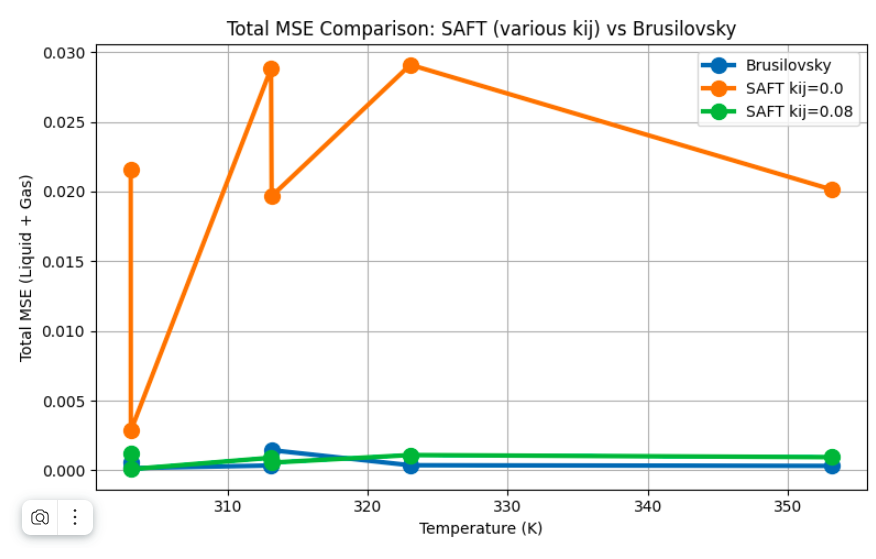
\includegraphics[width=\textwidth]{images/mole_hexane.png}
        \caption{$\mathrm{CO}_2$-гексан}
        \label{fig:rmse_hexane}
    \end{subfigure}
    \hfill
    \begin{subfigure}{0.30\textwidth}
        \centering
        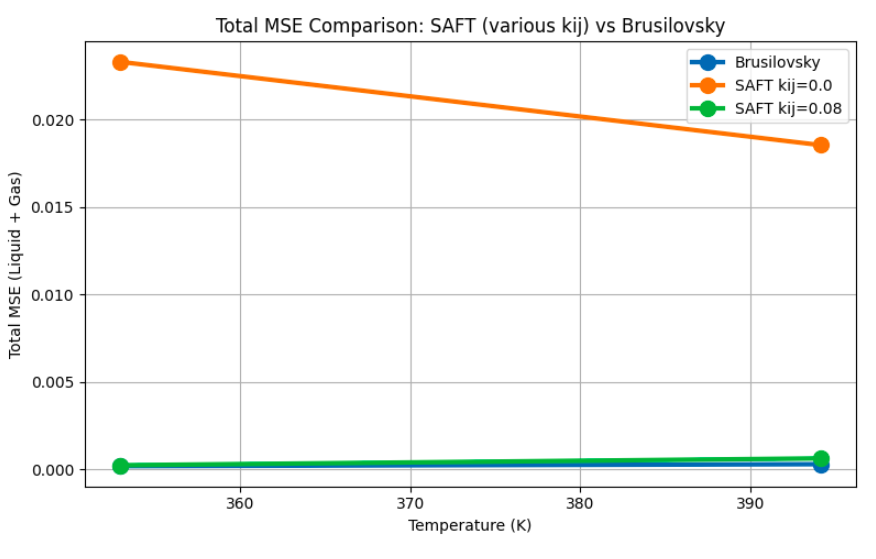
\includegraphics[width=\textwidth]{images/mole_heptane.png}
        \caption{$\mathrm{CO}_2$-гептан}
        \label{fig:rmse_heptane}
    \end{subfigure}
    \hfill
    \begin{subfigure}{0.30\textwidth}
        \centering
        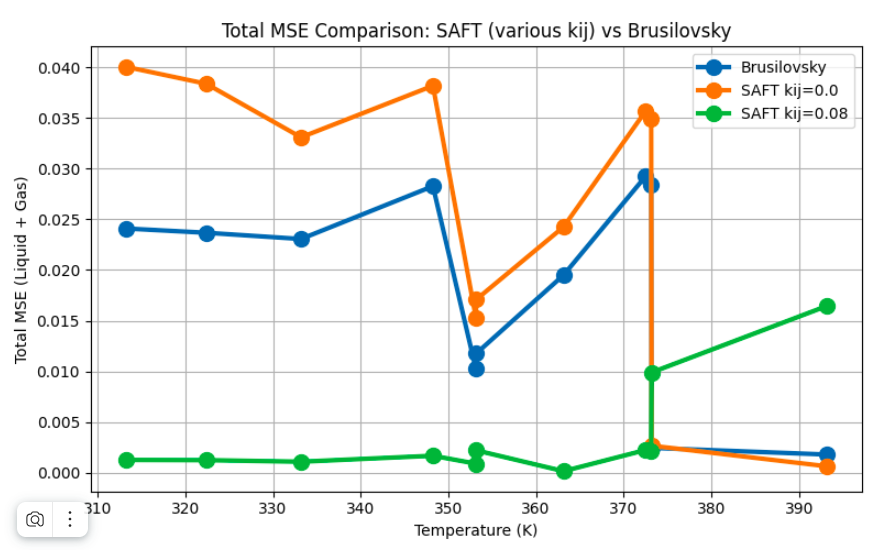
\includegraphics[width=\textwidth]{images/mole_octane.png}
        \caption{$\mathrm{CO}_2$-октан}
        \label{fig:rmse_octane}
    \end{subfigure}

    \vspace{0.5cm}

    % Second row
    \begin{subfigure}{0.30\textwidth}
        \centering
        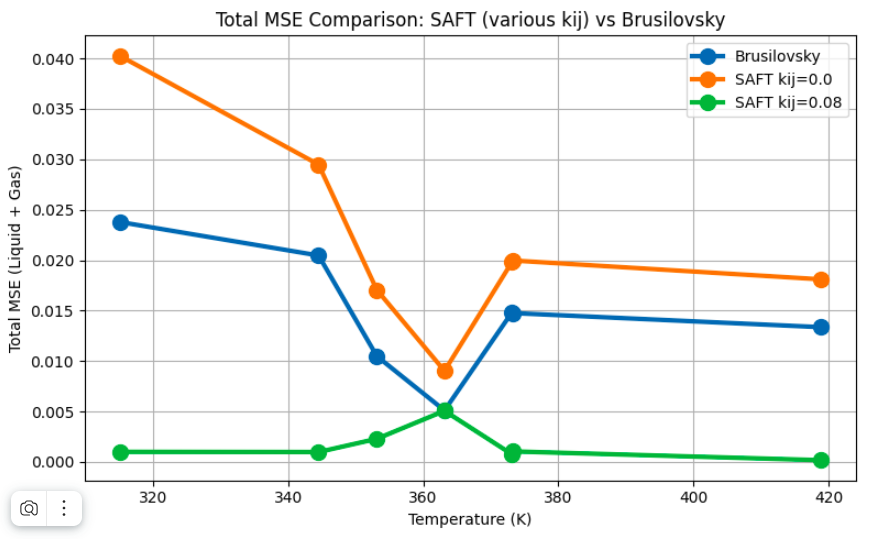
\includegraphics[width=\textwidth]{images/mole_nonane.png}
        \caption{$\mathrm{CO}_2$-нонан}
        \label{fig:rmse_nonane}
    \end{subfigure}
    \hfill
    \begin{subfigure}{0.30\textwidth}
        \centering
        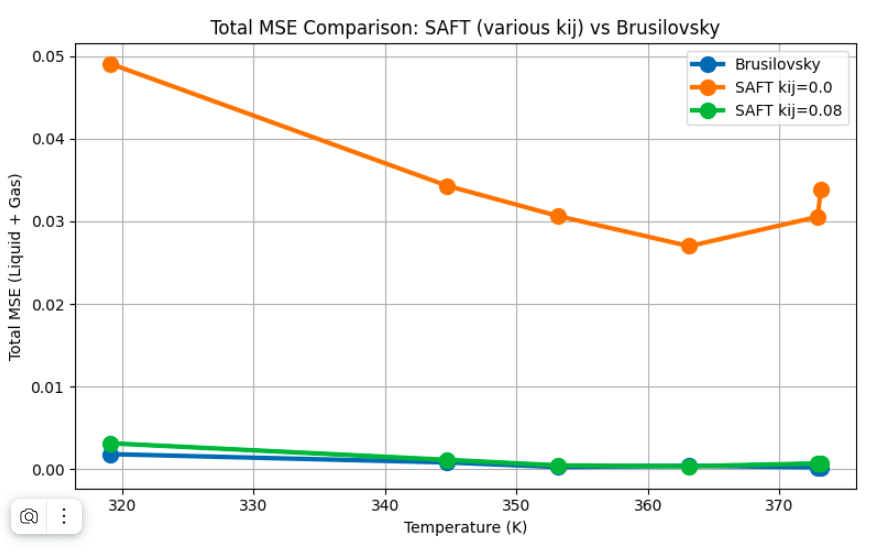
\includegraphics[width=\textwidth]{images/mole_decane.png}
        \caption{$\mathrm{CO}_2$-декан}
        \label{fig:rmse_decane}
    \end{subfigure}
    \hfill
    \begin{subfigure}{0.30\textwidth}
        \centering
        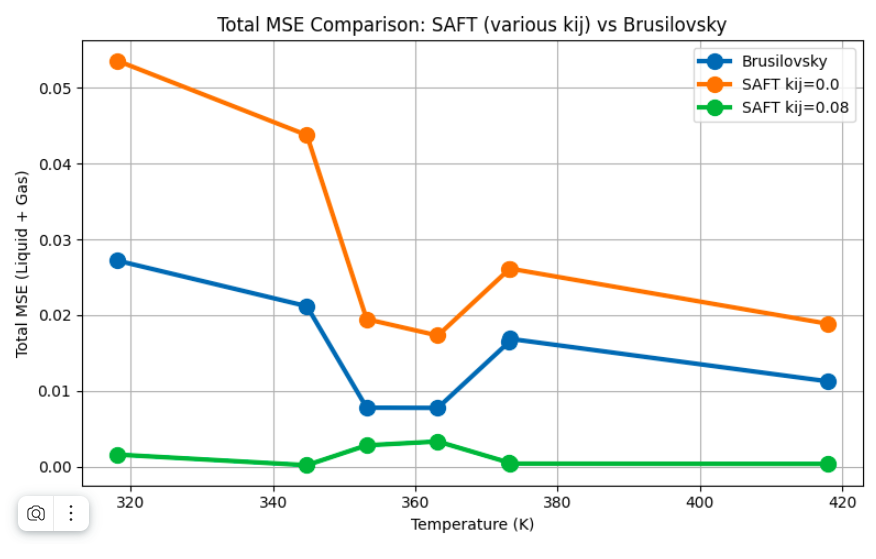
\includegraphics[width=\textwidth]{images/mole_dodecane.png}
        \caption{$\mathrm{CO}_2$-додекан}
        \label{fig:rmse_dodecane}
    \end{subfigure}

    \caption{Сравнение MSE мольной доли углекислого газа, предсказанной моделями Брусиловского и SAFT с оптимальным параметром \( k_{ij} \) и без него для различных систем $\mathrm{CO}_2$-алкан.}
    \label{fig:rmse_comparison}
\end{figure}
	
    \end{itemize}
    \item Анализ корреляций:
    \begin{itemize}
        \item Не выявлено устойчивой зависимости коэффициента \( k_{ij} \) от молекулярных параметров компонентов (длины цепи, размеров молекулы, глубины потенциальной ямы).
        \item Наблюдается слабая корреляция оптимальных значений \( k_{ij} \) с температурой и давлением.
    \end{itemize}
    \item Точность модели:
    \begin{itemize}
        \item Использование оптимизированных значений \( k_{ij} \) в CP-PC-SAFT позволило значительно улучшить точность предсказания фазового равновесия по сравнению с базовой версией модели.
    \end{itemize}
    \item Сравнение с уравнением состояния Брусиловского:
    \begin{itemize}
        \item В отдельных случаях CP-PC-SAFT с подобранными коэффициентами \( k_{ij} \) показала сопоставимую или лучшую точность предсказаний давления насыщения и состава фаз.
    \end{itemize}
    \item Оценка точности на тройных системах:
	\begin{itemize}
		\item В тройной системе $\mathrm{CO}_{2}$-бутан-декан точность улучшилась при использовании коэффициента парного взаимодействия $k_{ij} = 0$ между бутаном и $\mathrm{CO}_{2}$, поскольку данный случай не был параметризован. В похожем случае для уравнения Пенга-Робинсона \cite{Brusilovskii2002} упомянуто, что коэффициенты для алканов тяжелее пентана можно считать равными, тогда как для алканов легче коэффициент относительно мал.
	    \item Для системы $\mathrm{CO}_{2}$-декан бутан включение коэффициента $k_{ij} = 0.08$ между $\mathrm{CO}_{2}$ и деканом привело к минимальным значениям MAE и RMSE, подтверждая правильность подхода.
\begin{figure}[ht]
    \centering
    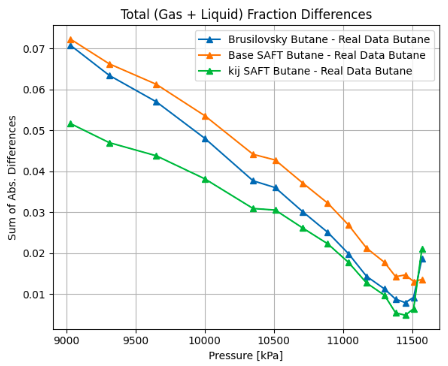
\includegraphics[width=0.4\textwidth]{images/3_butane_molar_liquid.png} % Укажи путь к файлу
    \caption{График ошибки в предсказании мольной доли бутана в смеси $\mathrm{CO}_{2}$-бутан-декан}
    \label{fig:3butane}
\end{figure}
	    \item В системах $\mathrm{CO}_{2}$-гексан-декан и $\mathrm{CO}_{2}$-октан-декан использование оптимизированных коэффициентов $k_{ij}$ значительно улучшило точность предсказания давления в точке кипения.
	    \item Для системы $\mathrm{CO}_{2}$-октан-декан модель CP-PC-SAFT с подобранными коэффициентами обеспечила более точные предсказания, чем уравнение состояния Брусиловского.
\begin{figure}[ht]
    \centering
    \begin{subfigure}{0.48\textwidth}
        \centering
        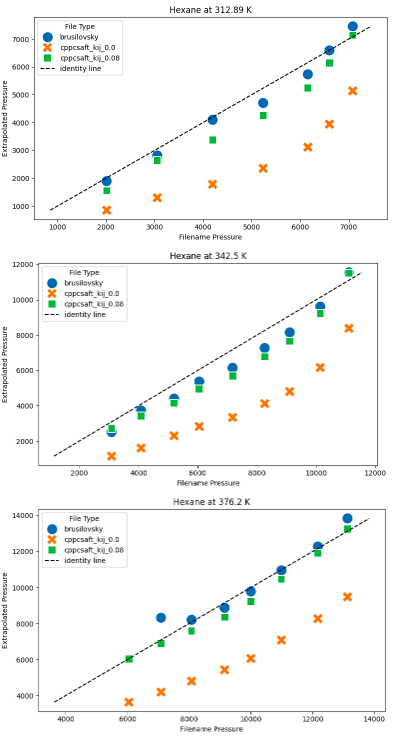
\includegraphics[width=\textwidth]{images/3_hexane_boiling.png} % Укажи правильный путь к файлу
        \caption{Предсказания давления кипения для смеси $\mathrm{CO}_2$-гексан-декан}
        \label{fig:accuracy_hexane}
    \end{subfigure}
    \quad
    \begin{subfigure}{0.48\textwidth}
        \centering
        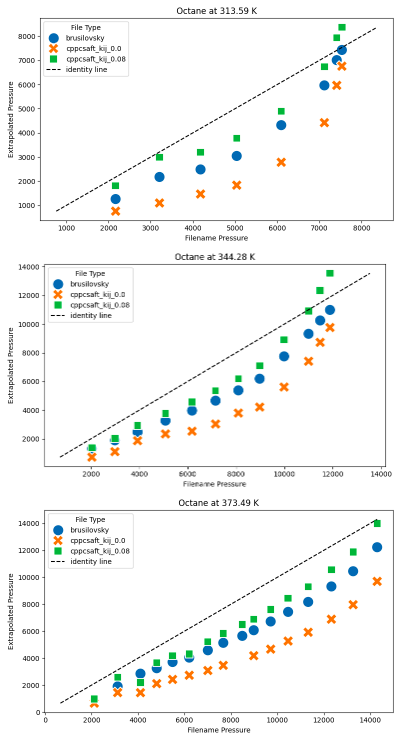
\includegraphics[width=\textwidth]{images/3_octane_boiling.png} % Укажи правильный путь к файлу
        \caption{Предсказания давления кипения для смеси $\mathrm{CO}_2$-октан-декан}
        \label{fig:accuracy_octane}
    \end{subfigure}
    \caption{Сравнение точности вычисления давления кипения в тройных системах}
    \label{fig:accuracy_comparison}
\end{figure}
	\end{itemize}
\end{itemize}


\subsection{Выводы}

Проведённый анализ и расчет коэффициентов парного взаимодействия \( k_{ij} \) для CP-PC-SAFT позволил улучшить качество предсказания фазового равновесия в смесях алкан–$\mathrm{CO}_{2}$.

Основные выводы исследования:
\begin{itemize}
    \item Оптимизированные коэффициенты \( k_{ij} \) обеспечивают точность, сопоставимую с промышленными моделями.
    \item Универсальная зависимость \( k_{ij} \) от параметров компонентов не выявлена, но предложенные значения позволяют значительно улучшить предсказания фазового состава.
    \item Разработанный подход может быть масштабирован на более сложные системы, включая трёхкомпонентные смеси.
\end{itemize}

В ходе работы освоен формат базы данных ThermoML и протестирована автоматизированная обработка экспериментальных данных, что открывает возможности дальнейшего применения данного метода в моделировании фазовых равновесий.

\section{Заключение}

\subsection{Краткие выводы}

В рамках проекта проведена параметризация коэффициентов парного взаимодействия \( k_{ij} \) для модели CP-PC-SAFT, что позволило повысить точность предсказания фазовых равновесий в смесях алкан–$\mathrm{CO}_{2}$.

\begin{itemize}
    \item Разработан рабочий подход к подбору коэффициентов \( k_{ij} \) на основе экспериментальных фазовых диаграмм.
    \item Оптимизированы значения \( k_{ij} \) для систем $\mathrm{CO}_{2}$ с алканами: гексан, гептан, октан, нонан, декан и додекан.
    \item Достигнута точность, сопоставимая с промышленными моделями, такими как уравнение состояния Брусиловского.
    \item Освоен формат базы данных ThermoML и разработан код для автоматизированной загрузки и предобработки экспериментальных данных.
    \item Разработанная методика позволяет адаптировать подход к другим веществам и типам смесей.
\end{itemize}

\subsection{Оценка полноты решений}

Проведённая работа позволила добиться существенного улучшения качества моделирования фазовых равновесий, однако остаются нерешённые вопросы:

\begin{itemize}
    \item Не обнаружена устойчивая зависимость коэффициента \( k_{ij} \) от параметров компонентов (длины цепи, размеров молекулы, глубины потенциальной ямы).
    \item Зафиксирована слабая корреляция оптимальных значений \( k_{ij} \) с температурой и давлением, но разброс данных не позволил предложить универсальную зависимость, превосходящую по точности использование константного значения \( k_{ij} \approx 0.08 \).
    \item Проверена обобщающая способность модели на трёхкомпонентных системах, однако метод требует дальнейшего тестирования для расширения применимости.
\end{itemize}

\subsection{Рекомендации по использованию}

Использование подобранных коэффициентов парного взаимодействия \( k_{ij} \) для CP-PC-SAFT рекомендуется в следующих случаях:

\begin{itemize}
    \item Предсказание фазового равновесия в смесях углеводородов с $\mathrm{CO}_{2}$, где предложенные коэффициенты обеспечивают более точные результаты.
    \item Расчёт давления насыщения при заданной температуре и составе жидкой фазы, с применением оптимизированных значений \( k_{ij} \).
    \item Расширение модели на системы с большим числом компонентов, с последующей корректировкой коэффициентов в зависимости от новых экспериментальных данных.
\end{itemize}

\subsection{Технико-экономическая эффективность внедрения}

Оптимизация коэффициентов парного взаимодействия \( k_{ij} \) в CP-PC-SAFT имеет ряд преимуществ:

\begin{itemize}
    \item Снижение потребности в трудоёмкой экспериментальной подгонке параметров модели, что сокращает время и затраты на анализ фазовых равновесий.
    \item Повышение точности предсказаний фазового состава позволяет оптимизировать процессы газоразделения и нефтехимической переработки, что ведёт к снижению расходов на технологические расчёты.
    \item Разработанный метод является гибким и может быть адаптирован к новым веществам и условиям, что увеличивает его ценность для практического применения.
\end{itemize}

\subsection{Оценка научно-технического уровня}

\begin{itemize}
    \item Разработанный подход к параметризации \( k_{ij} \) в CP-PC-SAFT соответствует современным тенденциям моделирования фазовых равновесий и конкурирует с промышленными моделями.
    \item Достигнутая точность сопоставима с уравнением состояния Брусиловского, что подтверждает эффективность предложенной параметризации.
    \item Созданная основа для масштабирования метода позволяет применять его для прогнозирования фазового равновесия в более сложных системах.
\end{itemize}

\newpage
\section*{Список использованных источников}
\printbibliography

\end{document}

